\chapter{Ansatz \& Implementierung}
\label{ansatz_und_implementierung}
Im Folgenden wird erläutert, wie vorgegangen wird, um die Fragestellung nach den Auswirkungen von Quantisierung und Pruning auf mobile Architekturen zu beantworten und wie die einzelnen Optimierungstechniken auf die ausgewählten Architekturen angewendet werden. Dazu wird im ersten Abschnitt beschrieben was das grundsätzliche Vorgehen in dieser Arbeit ist, um die verschiedenen Architekturen miteinander vergleichen zu können. Anschließend wird kurz die für die Implementierung verwendete Bibliothek TensorFlow erläutert. Im dritten Abschnitt werden die Trainingskonfiguration und der Datensatz beschrieben, mit denen alle Architekturen trainiert werden. Zum Schluss wird in den letzten beiden Abschnitten darauf eingegangen, wie genau die Quantisierung und das Pruning der vorgestellten Architekturen implementiert und durchgeführt werden.



\section{Vorgehen}
\label{vorgehen}
In dieser Arbeit wird grundsätzlich wie folgt vorgegangen: Als Erstes werden die im Abschnitt \ref{architekturen} vorgestellten Architekturen auf einem ausgewählten Datensatz trainiert und die trainierten Modelle gesichert.
Auf Basis dieser vortrainierten und gesicherten Modelle werden anschließend die Optimierungstechniken Quantisierung und Pruning angewendet. Dazu werden die Modelle immer ausgehend von den vortrainierten Modellen quantisiert, gepruned und sowohl zuerst gepruned als auch anschließend quantisiert. So ergeben sich die folgenden Kombinationen von Modelloptimierungen:

\begin{itemize}
\item vortrainiert
\item vortrainiert und quantisiert
\item vortrainiert und gepruned
\item vortrainiert, gepruned und quantisiert
\end{itemize}

Die 4 Kombinationen werden anschließend untereinander verglichen und es wird untersucht, was die Auswirkungen der architekturellen Besonderheiten der mobilen Architekturen unter Anwendung von Quantisierung und Pruning sind.



\section{TensorFlow}
Für die Implementierung wird die Python Bibliothek TensorFlow \footnote{\url{https://www.tensorflow.org/}} verwendet. TensorFlow stellt eine Reihe von Implementierungen verschiedener Netzwerke und Algorithmen des maschinellen Lernens bereit. Dazu gehören auch Implementierungen der in Abschnitt \ref{architekturen} vorgestellten Architekturen, was eine händische Implementierung dieser Architekturen überflüssig macht.


\subsection{TensorFlow Lite}
Um die Quantisierung von Modellen zu ermöglichen, bietet TensorFlow (\lstinline{tf}) ein Modul namens TensorFlow Lite (\lstinline{tf.lite}). Dieses Modul ist auf die Entwicklung von Modellen für mobile und eingebettete Systeme wie Mobiltelefone oder Mikrocontroller spezialisiert.
Implementiert ist in diesem Modul beispielsweise die Post-Training Quantisierung. Außerdem stellt TensorFlow Lite den TFLite FlatBuffer als effiziente Datenstruktur zum Speichern von Modellen zur Verfügung. Die TFLite FlatBuffer Datenstruktur ist eine optimierte Variante der FlatBuffer Bibliothek \footnote{\url{https://google.github.io/flatbuffers/flatbuffers\_white\_paper.html}}. Bei dem FlatBuffer Format handelt es sich um ein binäres Format, welches im Gegensatz zu z.B. JSON oder XML nicht menschenlesbar ist, aber dadurch mit wenig Overhead auskommt und aus diesem Grund besonders speicherplatzeffizient ist.
 

\subsection{TensorFlow Model Optimization Toolkit}
Für das Pruning wird zusätzlich noch das TensorFlow Model Optimization Toolkit \footnote{\url{https://www.tensorflow.org/model\_optimization}} benötigt. Diese Bibliothek stellt einige Algorithmen bereit, um Modelle des maschinellen Lernens zu optimieren. Dazu zählt beispielsweise das Quantization-Aware Training, welches in Abschnitt \ref{quantization_aware_training} beschrieben wurde und das Magnitude Pruning aus Abschnitt \ref{magnitude_pruning}.



\section{Training}
\label{training}
In dem weiteren Verlauf der Arbeit werden ausschließlich die Standardvarianten der vorgestellten Architekturen betrachtet. Das bedeutet, dass keine Variationen des Breitenmultiplikators beim MobileNet und beim MobileNetV2 betrachtet werden, da dies lediglich die Anzahl an Parametern variiert, aber nichts grundsätzlich an der Architektur ändert. Aus demselben Grund wird beim EfficientNet ebenfalls nur das EfficientNet-B0 betrachtet, da die Varianten EfficientNet-B1 bis EfficientNet-B7 lediglich mittels Compound Scaling skaliert wurden, aber keine neuen Architekturen darstellen. Damit werden im Folgenden die Architekturen MobileNet, MobileNetV2, MobileNetV3 Large, MobileNetV3 Small und EfficientNet-B0 verwendet.

Diese Architekturen werden bereits von der TensorFlow Bibliothek (\lstinline{tf}) in dem Modul \lstinline{tf.keras.applications} implementiert und können einfach instanziiert werden. Beim Erzeugen einer Instanz dieser Architekturen kann über den \lstinline{weights}-Parameter angegeben werden, ob die Architektur mit vortrainierten Gewichten geladen werden soll oder ob lediglich eine zufällige Initialisierung der Gewichte erfolgen soll. Die vortrainieren Gewichte sind auf dem ImageNet Datensatz \cite{russakovsky_imagenet_2015} vortrainiert. Jedoch unterstützen die auf ImageNet vortrainierten MobileNet Architekturen keine Eingaben der Größe $32 \times 32 \times 3$ wie es bei dem verwendeten CIFAR-10 Datensatz (siehe Abschnitt \ref{datensatz}) der Fall ist. Aus diesem Grund werden in dieser Arbeit die Architekturen mit zufällig initialisierten Gewichten neu trainiert.

Um ein möglichst einheitliches Trainings-Setup für alle Architekturen zu schaffen, werden alle Architekturen mit denselben Trainingsparametern trainiert. Für die Trainingsdurchläufe wird der von allen vorgestellten Architekturen vorgeschlagene RMSprop Optimizer (\lstinline{tf.keras.optimizers.RMSprop}) \cite{howard_mobilenets_2017, sandler_mobilenetv2_2019, howard_searching_2019, tan_efficientnet_2020} mit einem Momentum von 0.9 verwendet. Da es sich bei der Aufgabe, welche die Netzwerke lernen sollen, um ein Klassifizierungsproblem mit mehr als zwei Klassen handelt, wird die Categorical Cross-Entropy Verlustfunktion (\lstinline{tf.keras.losses.CategoricalCrossentropy}) gewählt. Als Batch Size wird 64 verwendet. Die Learning Rate wird während des Trainings in 150 Epochen, beginnend bei einer initialen Learning Rate von $1 \cdot 10^{-3}$, linear auf 0 abgesenkt (\lstinline{tf.keras.optimizers.schedules.PolynomialDecay}). Diese Wahl der Parameter hat in der Arbeit am besten funktioniert, um alle Architekturen mit denselben Parametern trainieren zu können. Um ein Overfitting der Modelle während des Trainings abzumildern, wird das Training mittels EarlyStopping abgebrochen, wenn beim Training innerhalb von 50 Epochen keine Verbesserung des Verlustes auf den Testdaten erreicht wird (\lstinline{tf.keras.callbacks.EarlyStopping}).

Am Ende jedes Trainings wird das trainierte Modell abgespeichert, um in späteren Schritten ein Pruning oder eine Quantisierung darauf anzuwenden.


\subsection{Datensatz}
\label{datensatz}
Als Datensatz wird in dieser Arbeit der CIFAR-10 Datensatz \cite{krizhevsky_learning_2009} verwendet. Dieser Datensatz enthält insgesamt 60000 Farbbilder der Größe $32 \times 32$ Pixel. Die Bilder in dem Datensatz können in 10 Klassen eingeordnet werden: Flugzeug, Automobil, Vogel, Katze, Hirsch, Hund, Frosch, Pferd, Schiff und Lastkraftwagen. Zu jeder dieser Kategorien sind jeweils 6000 Bilder in dem Datensatz vorhanden. Der gesamte Datensatz ist zusätzlich noch aufgeteilt in eine Trainingsmenge und eine Testmenge. Die Trainingsmenge enthält insgesamt 50000 Bilder mit jeweils 5000 Bildern pro Klasse und die Testmenge enthält die restlichen 10000 Bilder. In Abbildung \ref{f3.1} ist je ein Beispielbild für jede Klasse dargestellt.

\begin{figure}[htbp]
\centerline{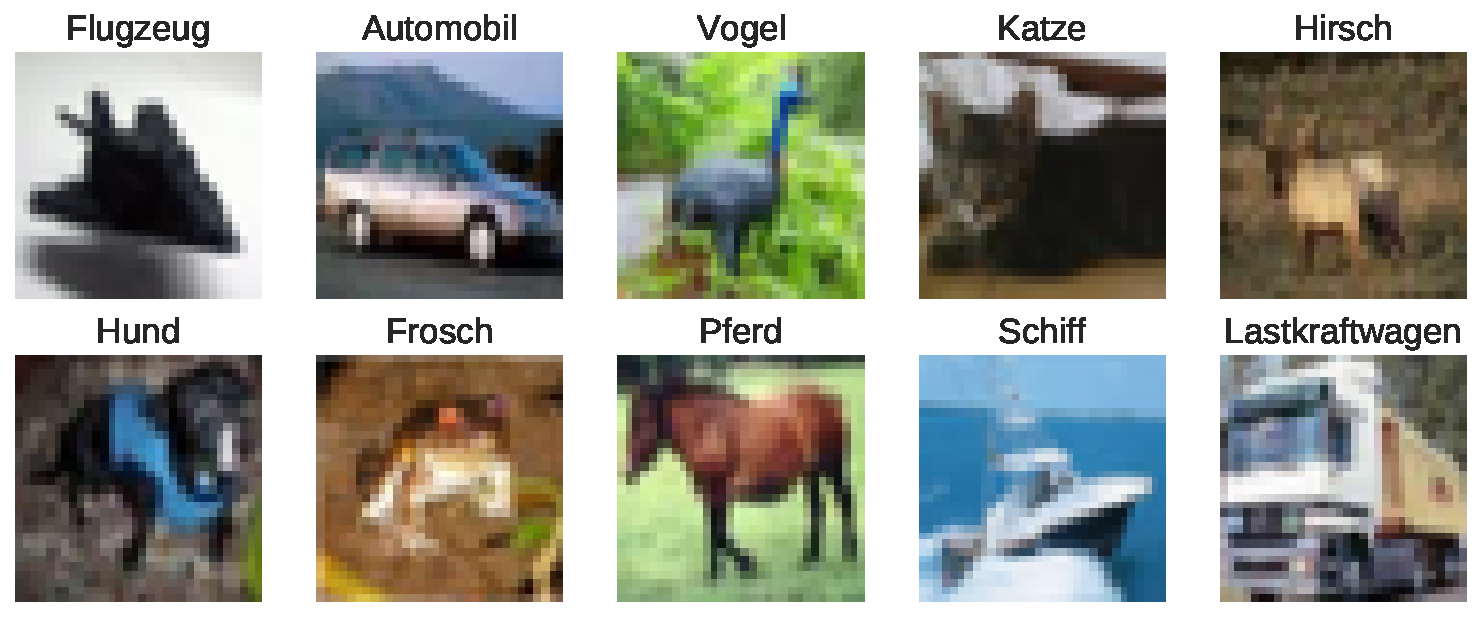
\includegraphics[width=0.8\textwidth]{content/images/cifar-10.pdf}}
\caption{Ein Beispielbild pro Klasse aus dem CIFAR-10 Datensatz.}
\label{f3.1}
\end{figure}

Der Grund, warum für diese Arbeit der CIFAR-10 Datensatz gewählt wurde, ist, dass für die Vergleiche der verschiedenen Architekturen untereinander und das Pruning viele Trainingsdurchläufe benötigt werden. Durch die geringe Anzahl und niedrige Auflösung der Bilder des CIFAR-10 Datensatzes ist ein einfaches Training möglich. Der häufig in der Literatur verwendete ImageNet Datensatz \cite{russakovsky_imagenet_2015} hingegen enthält insgesamt 1431167 hochauflösende Bilder und ist somit für diese Arbeit ungeeignet, da dieser durch die enorme Datenmenge die für diese Arbeit verfügbaren Kapazitäten überschreitet.



\section{Quantisierung}
\label{impl_quantisierung}
Zu der Quantisierung wurde in Abschnitt \ref{quantisierung} sowohl die Post-Training Quantisierung als auch das Quantization-Aware Training erläutert. Beim Quantization-Aware Training werden Modelle mittels simulierter Quantisierung von Grund auf trainiert. Hingegen kann die Post-Training Quantisierung direkt auf bereits trainierte Modelle angewendet werden, ohne ein erneutes Training zu erfordern. Aus zeitlichen Gründen wird in dieser Arbeit vorrangig die Post-Training Quantisierung betrachtet.

Ausgehend von einem 32 Bit Fließkomma Modell bietet TensorFlow für die Post-Training Quantisierung im Wesentlichen 3 Methoden an. Das ist zum einen die Post-Training Dynamic Range Quantization, bei der die Parameter des Modells lediglich für die Speicherung quantisiert werden und zur Inferenzzeit wieder in 32 Bit Fließkommazahlen konvertiert werden. Eine weitere Option die TensorFlow bietet ist das Quantisieren der Parameter in 16 Bit Fließkommazahlen. Als dritte Option bietet TensorFlow die Post-Training Integer Quantization an. Dazu gehört zum einen die Integer-Only Quantisierung, welche sämtliche Parameter und Aktivierungen in 8-Bit Integer quantisiert. Diese Integer-Only Quantisierung ist besonders wichtig für Hardware, welche nur Integer-Operationen unterstützt. Ein Beispiel für eine solche Integer-Only Hardware ist Googles Edge TPU \footnote{\url{https://cloud.google.com/edge-tpu}}. Zum anderen gehört zur Post-Training Integer Quantisierung auch die Float Fallback Quantisierung, welche ebenfalls wie die Integer-Only Quantisierung sämtliche Parameter und Aktivierungen in 8 Bit Integer quantisiert und lediglich die Ein- und Ausgabeschicht der Modelle im 32 Bit Fließkommaformat beibehält. In dieser Arbeit wird vorrangig die Post-Training Float Fallback Quantisierung betrachtet, da die EfficientNet Architekturen in TensorFlow derzeit noch nicht kompatibel mit der Integer-Only Quantisierung sind und durch die Quantisierung in 8 Bit Integer eine höhere Kompression der Modelle möglich ist als bei der Quantisierung in 16 Bit Fließkommazahlen.

Um diese Quantisierung durchzuführen stellt das TensorFlow Lite Modul den TFLiteConverter zur Verfügung (\lstinline{tf.lite.TFLiteConverter}). Eine Instanz dieses Konverters kann beispielsweise mit der Funktion \lstinline{tf.lite.TFLiteConverter.from_keras_model} erzeugt werden, welche als Parameter eine Instanz eines Keras Modells erwartet. Um dem erzeugten Konverter-Objekt mitzuteilen, dass das Modell quantisiert werden soll, muss das \lstinline{optimizations} Attribut des Objekts auf die Liste \lstinline{[ tf.lite.Optimize.DEFAULT ]} gesetzt werden. Für eine Float Fallback Quantisierung muss diesem erzeugten Konverter-Objekt zusätzlich ein repräsentativer Datensatz bekannt gemacht werden. Dieser repräsentative Datensatz sollte groß genug sein, um typische Werte für die Eingabedaten zu enthalten. Dabei kann es sich aber einfach um eine Untermenge der Trainingsdaten handeln. Der Datensatz wird anschließend von dem Konverter für Optimierungen bei der Quantisierung genutzt, wie beispielsweise das Vorhersehen von Wertebereichen der Eingabedaten. Anschließend kann auf dem Konverter-Objekt die \lstinline{convert()} Funktion aufgerufen werden, was letztendlich die Quantisierung und Konvertierung in das TFLite Format durchführt. Das resultierende TFLite Objekt kann anschließend als \lstinline{.tflite}-Datei gespeichert werden.

Neben der Quantisierung ist es mit dem \lstinline{TFLiteConverter} ebenfalls möglich trainierte Modelle ohne Anwendung von Quantisierung in das TFLite FlatBuffer Format zu konvertieren. Dazu muss erneut eine Instanz der Klasse \lstinline{tf.lite.TFLiteConverter} erstellt werden. Darauf muss anschließend direkt die \lstinline{convert()} Funktion aufgerufen werden, ohne irgendwelche Optimierungen zu spezifizieren.

Um eine Inferenz auf einem gespeicherten TFLite Modell durchzuführen, muss der TensorFlow Lite Interpreter (\lstinline{tf.lite.Interpreter}) verwendet werden. Dieser wird mit dem Pfad zu dem gespeicherten TFLite Modell instanziiert. Anschließend können mittels dieses Objektes Inferenzen auf dem geladenen Modell durchgeführt werden.



\section{Pruning}
\label{impl_pruning}
Das Pruning wird auf Grundlage der in Abschnitt \ref{training} trainierten Modelle durchgeführt. Dazu werden die Modelle geladen und erneut trainiert, wobei bei dem Training in regelmäßigen Abständen Gewichte auf 0 gesetzt werden. Dieses Pruning erfolgt nach dem Konzept des Magnitude Pruning, welches in Abschnitt \ref{magnitude_pruning} beschrieben wurde. Dazu wird das TensorFlow Model Optimization Toolkit (\lstinline{tfmot}) verwendet, welches in dem Modul \lstinline{tfmot.sparsity.keras} sämtliche Funktionalitäten enthält, um ein Magnitude Pruning durchzuführen.

Für das Magnitude Pruning nach dem TensorFlow Model Optimization Toolkit muss als Erstes jedes zu prunende Layer mit der Funktion \lstinline{prune_low_magnitude} aus dem Modul \lstinline{tfmot.sparsity.keras} markiert werden. Diese Funktion erwartet eine Schicht, die gepruned werden soll und zusätzlich ein \lstinline{PruningSchedule} Objekt, welches beschreibt, wie der Pruningprozess ablaufen soll. Diese Arbeit verwendet hier das in Abschnitt \ref{magnitude_pruning} beschriebene schrittweise Pruning, das mittels \lstinline{tfmot.sparsity.keras.PolynomialDecay} als \lstinline{PruningSchedule} Objekt implementiert wurde. Um nun jede Schicht mit der Funktion \lstinline{prune_low_magnitude} zu markieren, wird die \lstinline{tf.keras.models.clone_model} Funktion verwendet, welche ein Modell und eine Funktion als Parameter entgegennimmt und als Ergebnis ein neues Modell zurück gibt, welches durch die Funktionsanwendung der gegebenen Funktion auf jede Schicht des gegebenen Modells entstanden ist.

Mit dieser Methodik können die MobileNet und MobileNetV2 Architekturen ohne Probleme für das Magnitude Pruning vorbereitet werden, indem als übergebene Funktion für die \lstinline{tf.keras.models.clone_model} Funktion lediglich die \lstinline{prune_low_magnitude} Funktion verwendet wird. Jedoch treten bei den MobileNetV3 und EfficientNet Architekturen Probleme auf, da bei diesen Architekturen Schichten verwendet werden, welche in TensorFlow nicht gepruned werden können. Dabei handelt es sich um die Schichten der folgenden Klassen:

\begin{itemize}
\item \lstinline{tf.python.keras.layers.preprocessing.image_preprocessing.Rescaling}
\item \lstinline{tf.python.keras.layers.preprocessing.normalization.Normalization}
\item \lstinline{tf.python.keras.layers.core.TFOpLambda}
\end{itemize}

Bis auf die \lstinline{Normalization} Schicht tragen die beiden anderen Klassen von Schichten keinerlei Parameter zu den Architekturen bei und haben somit auch keine Parameter die gepruned werden können. Die \lstinline{Normalization} Schicht der EfficientNet Architekturen trägt 7 Parameter zur Gesamtarchitektur bei, was wegen der geringfügigen Menge im Folgenden vernachlässigt wird. Um nun ein Pruning der MobileNetV3 und EfficientNet Architekturen zu ermöglichen, wurde eine eigene Methode (\lstinline{prune_model.prune_layer}) um die \lstinline{prune_low_magnitude} Funktion geschrieben, welche es ermöglicht, neben der zu prunenden Schicht und dem \lstinline{PruningSchedule} Objekt, einen zusätzlichen regulären Ausdruck anzugeben. Mit diesem regulären Ausdruck können Schichten, dessen Namen auf den regulären Ausdruck zutreffen vom Pruning ausgeschlossen werden. Mit dieser Funktion ist es nun möglich alle Architekturen für das Pruning zu markieren und zusätzlich falls erforderlich durch den regulären Ausdruck gezielt Schichten vom Pruning auszuschließen.

In dieser Arbeit werden beim Pruning für jede Architektur 30\%, 60\% und 90\% Sparsity (Anteil der auf 0 gesetzten Gewichte) betrachtet. Um die gewünschte Sparsity zu erreichen, läuft der Pruningprozess nach dem schrittweise Pruningalgorithmus ab, welcher mit der Formel \ref{f2.8} beschrieben wird. Für jeden Prozentsatz auf 0 gesetzter Gewichte werden andere Parameter für den schrittweisen Pruningalgorithmus benötigt, um ein Overfitting der Modelle bei geringer Sparsity durch zu viele Pruningschritte zu verhindern und schlecht trainierte Modelle durch zu wenige Pruningschritte bei hoher Sparsity zu vermeiden. Die verwendeten Parameter für die unterschiedlichen finalen Sparsity-Werte sind in Tabelle \ref{t3.1} dargestellt.

\begin{table}[ht]
\centering
\begin{tabular}{l|c|ccc}
                           &            & 30\% & 60\% & 90\% \\
\hline
Initiale Sparsity          & $s_i$      & 0    & 0    & 0    \\
Finale Sparsity            & $s_f$      & 0.3  & 0.6  & 0.9  \\
Startzeitpunt in Epochen   & $t_0$      & 0    & 0    & 0    \\
Frequenz in Epochen        & $\Delta t$ & 1    & 2    & 6    \\
Anzahl der Pruningschritte & $n$        & 2    & 3    & 4    \\
\end{tabular}
\caption{Verwendete Parameter für den schrittweisen Pruningalgorithmus nach Formel \ref{f2.8} für 30\%, 60\% und 90\% auf 0 gesetzte Gewichte}
\label{t3.1}
\end{table}

Um das Pruning anzuwenden, muss ein erneutes Training auf den geladenen und bereits vortrainierten Modellen erfolgen, bei dem schrittweise Gewichte auf 0 gesetzt werden. Für dieses Training wird genau wie in Abschnitt \ref{training} als der Wert 64 als Batch Size verwendet. Außerdem wird auch hier als Optimizer der RMSprop Algorithmus mit einem Momentum von 0.9 verwendet. Die Anzahl an Epochen für das Training ergibt sich aus den Parametern in Tabelle \ref{t3.1} durch $t_0 + n \Delta t$. Die Learning Rate wird genau wie beim Training in Abschnitt \ref{training} im Verlauf des Pruningprozesses linear abgesenkt. Als initiale Learning Rate wird nach dem Paper \cite{zhu_prune_2017} eine um das 10-fache verringerte Learning Rate als beim normalen Training der Modelle verwendet. Das bedeutet die initiale Learning Rate beträgt $1 \cdot 10^{-4}$ und wird im Verlauf des Pruningvorgangs linear auf $1 \cdot 10^{-5}$ abgesenkt.

Nach dem Pruningvorgang werden die geprunten Modelle gespeichert.



\section{Einheitliches Format für alle Modelle}
Um bei der Evaluation in Kapitel \ref{evaluation} ein einheitliches Format für alle Modelle zu verwenden, wird jedes Modell vor der Evaluation in das TFLite FlatBuffer Format konvertiert. Die Konvertierung in das TFLite FlatBuffer Format erfolgt, wie am Ende des Abschnitt \ref{impl_quantisierung} beschrieben, mithilfe des \lstinline{TFLiteConverter} (\lstinline{tf.lite.TFLiteConverter}).